%! Author = Runge
%! Date = 29-12-2023

% Preamble
\documentclass[a4paper,conference]{IEEEtran}

% Packages
%! Author = Runge
%! Date = 29-12-2023

% Packages
\RequirePackage{clrscode4e}
\usepackage{amsmath}
% \usepackage{amsthm} \\ the proof environment clashes with the one in pf2.
\usepackage{amssymb}
\usepackage{amsbsy}
\usepackage{mathrsfs}
\usepackage{dsfont}
\usepackage{bbold}
\usepackage{booktabs}
\usepackage{tikz}
\usepackage{pf2}
\usepackage{thmtools, thm-restate}
\usepackage{stmaryrd}
\usepackage{mathabx}
\usepackage{algpseudocode}

% Packages with options set
\usepackage[hidelinks]{hyperref}
\usepackage[textsize=small,obeyDraft]{todonotes}
\usepackage[newfloat]{minted}
\usepackage[backend=biber,
    bibencoding=utf8,
    maxbibnames=20,
    style=ieee,
    citestyle=numeric-comp,
    url=false
]{biblatex}
\usepackage[acronym]{glossaries}

% Package setup
\setlength{\marginparwidth}{2cm} % todonotes width
\setminted{linenos, autogobble, breaklines, fontsize=\footnotesize, style=friendly, xleftmargin=1em, numbersep=5pt}
\addbibresource{bib/main.bib}

% Other setup and options
\declaretheorem{theorem}
\declaretheorem{lemma}
\declaretheorem{definition}
\declaretheorem{example}
\declaretheorem{conjecture}
\newfloat{algorithm}{htb!}{lop}
\floatname{algorithm}{Algorithm}
\newcommand{\algorithmautorefname}{Algorithm}

\makeatletter
\providecommand{\bigsqcap}{%
  \mathop{%
    \mathpalette\@updown\bigsqcup
  }%
}
\newcommand*{\@updown}[2]{%
  \rotatebox[origin=c]{180}{$\m@th#1#2$}%
}
\makeatother

\makeglossaries

\tikzstyle{state} = [rectangle, minimum width=1.5cm, minimum height=1cm, text centered, draw=black, fill=white!30]
\tikzstyle{circle} = [ellipse, minimum width=1.5cm, minimum height=0.5cm, text centered, draw=black, fill=white!30]

\newcommand{\abssem}[1]{S^\# \llbracket #1 \rrbracket}
\newcommand{\absexpsem}[1]{E^\# \llbracket #1 \rrbracket}
\newcommand{\env}[1]{\rho_{#1}}
\newcommand{\abstable}{t^\#}
\newcommand{\abstablep}{t'^{\#}}
\newcommand{\absvars}{a^\#}
\newcommand{\absattrs}{\overset{\rightarrow}{v_d^\#}}
\newcommand{\absattr}{x^\#}
\newcommand{\absexps}{\overset{\rightarrow}{e^\#}}
\newcommand{\absexp}[1]{e^\#_{#1}}
\newcommand{\abspred}{\phi^\#}
\newcommand{\clattice}[2]{C_{#1}(#2)}
\newcommand{\concrete}{\gamma}
\newcommand{\aabstract}{\alpha}
\DeclareMathOperator{\map}{map}

\input{setup/acronyms}
%! Author = Runge
%! Date = 29-12-2023

\title{SQAAL - Extending and Simplifying Abstract Interpretation of Structured Query Language}

\author{\IEEEauthorblockN{
    Anders Malta Jakobsen\IEEEauthorrefmark{1},
    Casper Ståhl\IEEEauthorrefmark{2},
    Daniel Runge Petersen\IEEEauthorrefmark{3} \\
    Lars Emanuel Hansen\IEEEauthorrefmark{4},
    Oliver Holmgaard\IEEEauthorrefmark{5} and
    Sebastian Aaholm\IEEEauthorrefmark{6}}
\IEEEauthorblockA{Dept. of Computer Science,
    Aalborg University\\
    Aalborg, Denmark\\
    Email: \IEEEauthorrefmark{1}amja23,
    \IEEEauthorrefmark{2}cstahl20,
    \IEEEauthorrefmark{3}dpet20,
    \IEEEauthorrefmark{4}leha20,
    \IEEEauthorrefmark{5}oholmg20,
    \IEEEauthorrefmark{6}saahol20\\ @student.aau.dk}}


% Document
\begin{document}
    \maketitle
    %! Author = Runge
%! Date = 29-12-2023

\IEEEtitleabstractindextext{%
    \begin{abstract}
        This paper presents an extension of abstract interpretation applied to SQL, aiming to overcome the non-termination problem in Halder and Cortesi's work.
        Our method resolves this non-termination issue by introducing additional abstractions for both tuples and values.
        Additionally, we introduce new abstractions of the values using regular expressions for strings and intervals for integers, which we have seen mentioned by Cousot but have yet to find any papers on or implementations for.
        Our framework is informally proven to be sound and terminate reliably, providing a solid foundation for future research.
    \end{abstract}
    \begin{IEEEkeywords}
        Abstract Interpretation, Databases, Formal Verification, Program Analysis
    \end{IEEEkeywords}
}
    %! Author = Runge
%! Date = 29-12-2023

\section{Introduction}\label{sec:introduction}
%background and motivation
Abstract interpretation, first proposed by Cousot and Cousot in 1977~\cite{cousot_abstract_1977}, has emerged as a fundamental method for static program analysis.
Over the years, it has evolved into a versatile tool, finding applications across various programming paradigms and system architectures.
Its utility extends beyond traditional imperative programming to encompass object-oriented designs and concurrent systems~\cite{gustafsson_analyzing_2013, mine_static_2023}.
Abstract interpretation has played a pivotal role in analyzing a spectrum of program properties, from basic safety and liveness concerns to intricate security considerations~\cite{mastroeni_abstract_2011}.


Building upon this historical foundation, subsequent researchers, such as Halder and Cortesi, have expanded the application of abstract interpretation to domains like query languages \cite{halder_abstract_2012}.
This paper continues in the footsteps of these pioneers, aiming to further explore and extend the capabilities of abstract interpretation within the context of query languages.

%Objective
\todo[inline]{I think we should be more specific about the objective. This is not done}
The objective of this work is to develop a general software tool, in the sense of value analysis, only be considering abstract values, not meta information like information flow or taint analysis.
Within this limitation we will restrict try to pick the most abstract/powerfull primitives possible, that do not encounter computation problems.
Utilizing abstract interpretation for analyzing the reachable state space of an entity relation database given its schema, accompanying reactive procedures and a model of the behavior of the environment in which the database will reside.


\todo[inline]{Maybe we can use workflow nets for the environment behavior model.}

This research endeavor is motivated by the observation that, despite the widespread use of abstract interpretation in program analysis, there is a notable absence of a comprehensive, general-purpose tool tailored specifically for value analysis in query languages.
The lack of such a tool represents a significant gap in the field, hindering researchers and practitioners from effectively analyzing and verifying complex systems.
By addressing this gap, our work seeks to provide a valuable contribution to the field of program analysis, enabling more efficient and accurate evaluation of software systems.
\paragraph{Justification}

It seems that no general tool has been developed.


\section{Notes}
\paragraph{Guidance to the reader}

\begin{itemize}
    \item The reader should have a basic understanding of SQL.
    \item The reader should understand abstract interpretation and whatever semantics we are using.
    \item The reader should understand that a main contribution is a open source tool.
\end{itemize}

\paragraph{Conclusion}

\begin{itemize}
    \item A software tool of limited scope has been developed.
    \item The abstractions and concretizations from a Galios connection
    \item The analysis is show to be sound.
    \item The usability of the system is discussed but not tested with rigor. 
\end{itemize}








    \section{Related Works}\label{sec:related-works}

\todo[inline]{Casper says: The seminal work of \cite{cousot_abstract_1977} should also be mentioned here.}

\todo[inline]{Casper says: \cite{cousot_abstract_1996} should also be mentioned here, and maybe the fact that we try to \emph{implement} some of the ideas mentioned namely regular expressions as abstract domains and kindof linear inequalities and in that regard we should mention \cite{li2010abstract}.}

This paper builds on work of abstract interpretation of database queries by Cortesi and Halder~\cite{halder_abstract_2012}.
Concretely, we use their work for analysing a database schema in relation to a program using the syntax they describe.\todo[inline]{Casper says: the Related Works section should also give  brief outline of their contribution.}


Additionally, we use LTL as described in X, Y, and Z to describe properties to check against.\todo{Casper says: not anymore}

    
\section{preliminaries}\label{sec:preliminaries}

\subsection{Lattices}\label{subsec:lattices}
This section contains the definitions and theorems of lattices, complete lattices, and partial orders.
These definitions will be used later in the paper and are foundational to abstract interpretation.
All definitions and notation in this subsection are due to \cite{nielson_formal_2019}.

\begin{definition}
    A \emph{partial order} $(S, \sqsubseteq)$ is set $S$ equipped with a binary relation $\sqsubseteq$ that is reflexive, transitive and antisymmetric.
\end{definition}


For $X \sqsubseteq S$ and $y \in S$ we take


\begin{equation}
    X \sqsubseteq y \iff \forall x \in X : x \sqsubseteq y,
\end{equation}


and analogous for $y \sqsubseteq X$.


\begin{definition}
    A \emph{complete lattice} $(S, \sqsubseteq, \sqcup, \sqcap)$ is a partial order $(S, \sqsubseteq)$ in which for all $X \subseteq S:$ $\bigsqcup X$ and $\bigsqcap X$ are defined,
        \begin{equation}
            X \sqsubseteq \bigsqcup X \land \forall y \in S : X \sqsubseteq y \implies \bigsqcup X \sqsubseteq y,
        \end{equation}
        and
        \begin{equation}
            \bigsqcap X \sqsubseteq X \land \forall y \in S : y \sqsubseteq X \implies y \sqsubseteq \bigsqcap X.
        \end{equation}
\end{definition}


As a shorthand we take $x \sqcup y = \bigsqcup \{x, y\}$ and $x \sqcap y = \bigsqcap \{x, y\}$.


\begin{definition}
    A \emph{lattice} $(S, \sqsubseteq, \sqcup, \sqcap)$ is a partial order $(S, \sqsubseteq)$ in which for all $x,y \in S:$ $x \sqcup y$ and $x \sqcap y$ are defined,
        \begin{equation}
            \{x, y\} \sqsubseteq x \sqcup y \land \forall z \in S : \{x, y\} \sqsubseteq z \implies x \sqcup y \sqsubseteq z,
        \end{equation}
        and
        \begin{equation}
            x \sqcap y \sqsubseteq \{x, y\} \land \forall z \in S : z \sqsubseteq \{x, y\} \implies z \sqsubseteq x \sqcap y.
        \end{equation}
\end{definition}


\begin{theorem}\label{thm:kleene_finite}
    In a complete lattice $L$ with finite height, every monotone function $f : L \rightarrow L$ has a unique fixed point
    \begin{equation}
        lfp(f) = \bigsqcup\{f^n(\perp) \mid n \in \mathbb{N}\}
    \end{equation}.
\end{theorem}


\begin{theorem}
    If $L_1, L_2, \dots, L_n$ are complete lattices, then so is the product:
    \begin{equation}
        L_1 \times L_2 \times \dots L_n = \{(x_1, x_2, \dots x_n) \mid x_i \in L_i\}
    \end{equation}

    Where the order $\sqsubseteq$ is defined component-wise:

    \begin{align}
        \begin{split}
        (x_1, x_2, \dots, x_n) &\sqsubseteq (x_1', x_2', \dots, x_n') \\
        \iff
        \forall i &= 1, 2, \dots n : x_i \sqsubseteq x_i'
        \end{split}
    \end{align}
\end{theorem}

\begin{theorem}
    If $A$ is a set and $L$ a complete lattice, then $A \rightarrow L$ is a complete lattice when
    \begin{equation}
    \begin{split}
        f \sqsubseteq g \iff \forall a \in A : f(a) \sqsubseteq g(a) \\ \text{ where } f,g \in A \rightarrow L.\label{eq:equation-complete-lattice-theorem}
    \end{split}
    \end{equation}
\end{theorem}

\todo[inline]{
    Casper says:
    The four theorems above should have a source.
}

\subsection{Abstract Interpretation}\label{subsec:abstract-interpretation1}
Here we give a quick presentation abstract interpretation.
The presentation is heavily based on~\cite{nielson_formal_2019} with some additions from~\cite{moller_statitc_nodate}.
As the presentation is rudimentary we encourage the reader to review~\cite{noauthor_abstract_nodate} or~\cite{cousot_abstract_1996} for an introduction of the subject, and the respective chapters in~\cite{nielson_formal_2019} and~\cite{moller_statitc_nodate} for a more complete explanation or~\cite{cousot_abstract_1977} for the seminal work.


Because of the particular flavor of abstract interpretation we use uses program graphs instead of control flow graphs we justify the conversion here, to be more precise we justify the conversion of control flow construct defined in \cite{halder_abstract_2012} to program graphs.
This particular flavor of abstract interpretation was choose because it allowed us to be encode the control flow in the graph, allowing us to \emph{abstract} away details of control flow in our analysis specification.

\begin{definition}
    Given a set $\rho \in \mathfrak{E}$ of possible concrete program memories, and a set $\ab{\rho} \in \ab{\mathfrak{E}}$ of possible abstract program memories, related by a concretization function $\gamma : \mathcal{P}(\ab{\mathfrak{E}}) \rightarrow \mathcal{P}(\mathfrak{E})$.
    A concrete semantic over program instructs $I \in \mathbb{I}$, $\sem{\cdot} : \mathbb{I} \rightarrow \mathfrak{E} \rightarrow \mathfrak{E}$ and an abstract semantic $\abssem{\cdot} : \mathbb{I} \rightarrow \mathcal{P}(\ab{\mathfrak{E}}) \rightarrow \mathcal{P}(\ab{\mathfrak{E}})$, $\abssem{\cdot}$ is said to be \emph{sound} whenever:
    \begin{equation}
        \rho \in \concrete(\ab{E}) \land \sem{I}(m) = m' \implies m' \in \concrete(\abssem{I}(\ab{E}))\label{eq:equation}
    \end{equation}
\end{definition}


\begin{definition}\label{def:valid1}
    Given a program graph with vertices $Q$ and edges $E$, an assignment $A : Q \rightarrow \mathcal{P}(\ab{\mathfrak{E}})$, that assignment is said to be \emph{valid} if its the case that:
    \begin{itemize}
        \item $Q$ is a finite set of nodes,
        \item $I$ is a set of instructions,
        \item $q_\triangleright, q_\blacktriangleleft \in Q$ are the \emph{initial node} and \emph{final node}, respectively,
        \item and $E \subseteq Q \times \mathbb{I} \times Q$ is a finite set of \emph{edges}.
    \end{itemize}
    An edge $q_\circ \xrightarrow{I} q_\bullet$ has \emph{source} node $q_\circ$ and \emph{target} node $q_\bullet$ and is labeled with action $I$.
    Finally $q_\triangleright, q_\blacktriangleleft \in Q$ are distinct, and no edges are to have source $q_\blacktriangleleft$.
\end{definition}


Given the previously two definitions, if the initial abstract memories for the initial program point $\ab{E}_\triangleright$ is set such that $E_{\triangleright} \subseteq \concrete(\ab{E}_\triangleright)$, for concrete memories holding initially $E_{\triangleright}$ in the initial program point, the abstract semantics are sound and the analysis assignment is valid, then it can be shown that if $\rho \in \concrete(A(q_\circ))$ and $\langle q_\circ; \rho \rangle \xRightarrow{\omega^\star} \langle q_\bullet; \rho' \rangle$ then $\rho' \in \concrete(A(q_\bullet))$.
What that intuitively means is that the analysis assignment is a safe over approximation of the actual state-space of the program.
Valid analysis assignment can then readily be computed as explained in~\cite{nielson_formal_2019}.

% \begin{theorem}\label{thm:galoispre}
%     For $\gamma : L_1 \rightarrow L_2$ where $L_1$ and $L_2$ are complete lattices there exist a function $\alpha : L_2 \rightarrow L_1$ such that $\alpha$ and $\gamma$ forms a Galois connection if $\gamma\left(\bigsqcap B\right) = \bigsqcap_{b \in B}\gamma(b)$ for every $B \subseteq L_1$.
% \end{theorem}

\subsection{Converting Code Program Graph}\label{subsec:converting-code-program-graph}
This section will briefly cover how the program graph is created.
Creating a program graph from the code is already a proven concept.
Therefore, this paper will not delve into the details but inform the reader.
The book used to show that the concept of creating a program graph from code is a proven concept~\cite[see][chap 2.2]{nielson_formal_2019}.
A program graph consists of a finite set of nodes, initial and final nodes, actions, and edges.

These directed edges represent the program's flow, and the nodes represent its state.
The edges' actions are the atomic operations that the program can perform.
The initial node is the program's starting point, and the final node is the program's end.
We denote the program graph as $edges(q_{\circ} \rightsquigarrow q_{\bullet})\llbracket I \rrbracket$ where $q_{\circ}$ is the initial node, $q_{\bullet}$ is the final node, and $I$ is the instruction.

The program graph is created by parsing the code and creating nodes and edges that represent the flow of the code.
This process, while it may sound complex, is relatively straightforward.
For instance, if the code is only an assignment of a variable, there will be a node for the initial state before the variable is assigned, a node for the final state after the variable is assigned, and an edge between them that represents the action of the assignment.
This is written as the following equation:

\begin{equation}
    edges(q_{\circ} \rightsquigarrow q_{\bullet})\llbracket x\coloneqq a \rrbracket = \{(q_{\circ}, x\coloneqq a, q_{\bullet})\}\label{eq:equation3}
\end{equation}


$q_{\circ}$ is the initial node, $q_{\bullet}$ is the final node\coloneqq and $x\coloneqq a$ is the assignment.
This creates a set that represents the program graph, which can be seen in \autoref{fig:tikz-program-graph-assignment}.
This is a simple example, and the program graph can be more complex depending on the code, but the concept is the same.
Further examples can be found in~\cite[Figure 2.6]{nielson_formal_2019}.

\begin{figure}[htb!]
    \center
    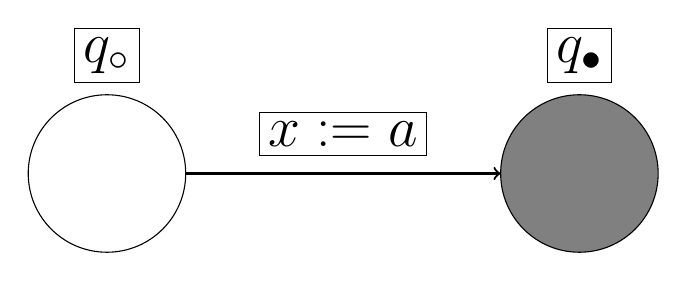
\begin{tikzpicture}
    \filldraw[fill=white, draw=black] (2,2) circle (1cm);
    \filldraw[fill=gray, draw=black] (8,2) circle (1cm);
    \node [draw] at (2,3.5) {\huge $q_{\circ}$};
    \node [draw] at (8,3.5) {\huge $q_{\bullet}$};
    \node [draw] at (5, 2.5) {\huge $x:=a$};
    \draw [thick, ->](3, 2) -- (7, 2);
\end{tikzpicture}
    \caption{An example that shows a program graph of an assignment}
    \label{fig:tikz-program-graph-assignment}
\end{figure}

We later describe the abstract syntax; \autoref{fig:abstract-syntax-instructions} describes the instructions the abstract syntax will contain.
There is no control structure in the abstract syntax, like if-statements and loops or sequences of instructions.
This is because the abstract syntax is simplified to make understanding the theory behind abstract interpretation easier.
This is all handled in the program graph, where the control structure is represented as edges in the program graph.

\begin{figure}
    \center
    \begin{tabular}{r l}
        $I \Coloneqq$ & $skip \mid v_a \coloneqq e \mid v_a \coloneqq ? \mid C_{sql} \mid b$
    \end{tabular}
    \caption{Abstract Syntax for Instructions}
    \label{fig:abstract-syntax-instructions}
\end{figure}

If-statements and loops are still used as boolean expressions in edges, used like guards in the program graph.
We can make equations for the edges of the program graph, where $b$ is a Boolean expression, and $S$ is a set of states done in the control structure.

For an if-statement `if b then S1 else S2`:
$edges(q_{\circ} \rightsquigarrow q_{\bullet})\llbracket \text{if } b \text{ then } S_1 \text{ else } S_2 \rrbracket = \text{let } q_{cond}, q_{if}, q_{else}, q_{merge}$ be new nodes.


\begin{align}
    \begin{split}
        S_{cond} &= edges(q_\circ \rightsquigarrow q_{if})\llbracket b \rrbracket \\
        & \cup edges(q_\circ \rightsquigarrow q_{else})\llbracket \neg b \rrbracket
    \end{split} \\
    S_{if} &= edges(q_{if} \rightsquigarrow q_{if_{out}})\llbracket S_1 \rrbracket \\
    S_{else} &= edges(q_{else} \rightsquigarrow q_{else_{out}})\llbracket S_2 \rrbracket \\
    S_{merge} &= edges(q_{if_{out}} \rightsquigarrow q_{\bullet}) \cup edges(q_{else_{out}} \rightsquigarrow q_{\bullet}) \\
    &\text{in } S_{cond} \cup S_{if_{in}} \cup S_{else_{in}} \cup S_{merge}
\end{align}

For a while loop `while b do I`:
$edges(q_{\circ} \rightsquigarrow q_{\bullet})\llbracket \text{while } b \text{ do } I \rrbracket = \text{let } q_{loop}$ be a new node.


\begin{align}
    I &\Coloneqq & &\texttt{if } b \texttt{ then } I_1 \texttt{ else } I_2 \\
      &\mid      & &\texttt{while } b \texttt{ do } I \\
      &\mid      & &I_1; I_2 \\
      &\mid      & &\dots
\end{align}

\begin{equation}
\begin{split}
    &edges(q_\circ \rightsquigarrow q_\bullet) \llbracket \texttt{if } b \texttt{ then } I_1 \texttt{ else } I_2 \rrbracket = \\
    &\quad \text{let } \\
    &\quad\quad q, q' \text{ be new nodes} \\
    &\quad\quad E_{b} = edges(q_\circ \rightsquigarrow q) \llbracket b \rrbracket \\
    &\quad\quad E_{\neg b} = edges(q_\circ \rightsquigarrow q') \llbracket \neg b \rrbracket \\
    &\quad\quad E_{I_1}= edges(q \rightsquigarrow q_\bullet) \llbracket I_1 \rrbracket \\
    &\quad\quad E_{I_2}= edges(q' \rightsquigarrow q_\bullet) \llbracket I_2 \rrbracket \\
    &\quad \text{in } E_{b} \cup E_{\neg b} \cup E_{I_1} \cup E_{I_2}
\end{split}\label{eq:equation14}
\end{equation}

In \autoref{fig:tikz-program-graph-loop} and \autoref{fig:tikz-program-graph-if}, we see examples of how a loop and an if-statement are represented in a program graph.


\begin{figure}[htb!]
    \center
    \begin{tikzpicture}
    \tikzstyle{arrow} = [thick,->,>=stealth]
    \node [circle, draw] (start) at (0,0){};
    \node [circle, draw, fill=black] (end) at (0,-2.3){};
    \node (a) [cloud,  cloud puffs=9.4, minimum width=1cm, draw, right=2cm of start, shift={($(start.south)+(0.2,-1cm)$)}] {$I_2$};
    \node (b) [cloud,  cloud puffs=9.4, minimum width=1cm, draw, left=2cm of start, shift={($(start.south)+(-0.2,-1cm)$)}] {$I_1$};

    \draw[arrow, ->] (start) to node[below,scale=.7,xshift=6, yshift=10] {$\neg b$} (a);
    \draw[arrow, ->] (start) to node[below,scale=.7,xshift=-4, yshift=10] {$b$} (b);
    \draw[arrow, ->] (a) to node[below,scale=.7] {} (end);
    \draw[arrow, ->] (b) to node[below,scale=.7] {} (end);
\end{tikzpicture}
    \caption{An example that shows a program graph of an if-statement}
    \label{fig:tikz-program-graph-if}
\end{figure}

\begin{equation}
\begin{aligned}
    &edges(q_\circ \rightsquigarrow q_\bullet) \llbracket \texttt{while } b \texttt{ do } I \rrbracket = \\
    &\quad \text{let } \\
    &\quad\quad q \text{ be new nodes} \\
    &\quad\quad E_{b} = edges(q_\circ \rightsquigarrow q) \llbracket b \rrbracket \\
    &\quad\quad E_{\neg b} = edges(q_\circ \rightsquigarrow q_\bullet) \llbracket \neg b \rrbracket \\
    &\quad\quad E_{I} = edges(q \rightsquigarrow q_\circ) \llbracket I \rrbracket \\
    &\quad \text{in } E_{b} \cup E_{\neg b} \cup E_{I}
\end{aligned}
\end{equation}

As visualized in \autoref{fig:tikz-program-graph-loop}.

\begin{figure}[htb!]
    \center
    \begin{tikzpicture}
    \tikzstyle{arrow} = [thick,->,>=stealth]
    \node (a) [cloud,  cloud puffs=9.4, minimum width=1cm, draw] {$I$};
    \node [circle, draw, above=of a] (start) {};
    \node [circle, draw, fill=black, below=of a] (end) {};

    \draw[arrow, ->] ([shift={(0.0,0.045)}]a.east) to[bend right] node[below,scale=.7] {} (start);
    \draw[arrow, ->] (start) -- node[right,scale=.70,xshift=-15]{b} (a);
    \draw[arrow, ->] (start) to[bend right=55] node[right,scale=.70,xshift=-20]{$\neg b$} (end);
\end{tikzpicture}
    \caption{An example that shows a program graph of a loop}
    \label{fig:tikz-program-graph-loop}
\end{figure}


In the abstract syntax, we will not have formulated sequences of $I_0, I_1, I_2, \dots, I_n$ as in the program graph, but rather as a set of states $S$, where we at the end go back to the initial state, as shown in \autoref{fig:tikz-composition-graph}.

We can make equations for the edges of the composition graph, where $I_1$ and $I_2$ are instructions:
$edges(q_{\circ} \rightsquigarrow q_{\bullet})\llbracket I_1 ; I_2 \rrbracket = $ let $q$ be a new node.


\begin{align}
    S_1 &= edges(q_{\circ} \rightsquigarrow q)\llbracket I_1 \rrbracket \\
    S_2 &= edges(q \rightsquigarrow q_{\bullet})\llbracket I_2 \rrbracket \\
    &\text{in } S_1 \cup S_2
\end{align}


\begin{figure}
    \center
    \begin{tikzpicture}
    \tikzstyle{arrow} = [thick,->,>=stealth]
    \node [circle, draw] (start) at (0,0){};
    \node (a) [cloud,  cloud puffs=9.4, minimum width=1cm, draw, shift={($(start.east)+(1.5,0)$)}] {$P_1$};
    \node [circle, draw, shift={($(a.east)+(1.5,0)$)}] (b) {};
    \node (c) [cloud,  cloud puffs=9.4, minimum width=1cm, draw, shift={($(b.east)+(1.5,0)$)}] {$P_2$};
    \node [circle, draw, shift={($(c.east)+(1.5,0)$)}, fill=black] (end) {};

    \draw[arrow, ->] (start) to node[above,scale=.7] {} (a);
    \draw[arrow, ->] (a) to node[above,scale=.7] {} (b);
    \draw[arrow, ->] (b) to node[above,scale=.7] {} (c);
    \draw[arrow, ->] (c) to node[above,scale=.7] {} (end);
\end{tikzpicture}

    \caption{An example that shows a composition graph}
    \label{fig:tikz-composition-graph}
\end{figure}

And when I is a base case, that is, not a sequential, if-else or while statement:
\begin{equation}
    edges(q_\circ \rightsquigarrow q_\bullet) \llbracket I \rrbracket = \{q_\circ \xrightarrow{I} q_\bullet\}
\end{equation}

Thus for some program $P = I$, the program graph of $P$ is simply $edges(q_\triangleright \rightsquigarrow q_\blacktriangleleft)\llbracket P \rrbracket$.

\subsection{Abstract Interpretation}\label{subsec:abstract-interpretation2}

Here we give a quick presentation abstract interpretation.
The presentation is heavily based on \cite{nielson_formal_2019} with some additions from \cite{moller_statitc_nodate}.
As the presentation is rudimentary we encourage the reader to review \cite{noauthor_abstract_nodate} or \cite{cousot_abstract_1996} for a informal introduction of the subject, and the respective chapters in \cite{nielson_formal_2019} and \cite{moller_statitc_nodate} for a more complete explanation or \cite{cousot_abstract_1977} for the seminal work.

First we define two central notions, namely soundness and valid analysis assignments.

\begin{definition}
    Given a set $\rho \in \mathfrak{E}$ of possible concrete program memories, and a set $\ab{\rho} \in \ab{\mathfrak{E}}$ of possible abstract program memories, related by a concretization function $\gamma : \mathcal{P}(\ab{\mathfrak{E}}) \rightarrow \mathcal{P}(\mathfrak{E})$.
    A concrete semantic over program instructs $I \in \mathbb{I}$, $\sem{\cdot} : \mathbb{I} \rightarrow \mathfrak{E} \rightarrow \mathfrak{E}$ and an abstract semantic $\abssem{\cdot} : \mathbb{I} \rightarrow \mathcal{P}(\ab{\mathfrak{E}}) \rightarrow \mathcal{P}(\ab{\mathfrak{E}})$, $\abssem{\cdot}$ is said to be \emph{sound} whenever:
    \begin{equation}
        \rho \in \concrete(\ab{E}) \land \sem{I}(m) = m' \implies m' \in \concrete(\abssem{I}(\ab{E}))
    \end{equation}
\end{definition}

\begin{definition}\label{def:valid2}
    Given a program graph with vertices $Q$ and edges $E$, an assignment $A : Q \rightarrow \mathcal{P}(\ab{\mathfrak{E}})$, that assignment is said to be \emph{valid} if its the case that:
    \begin{itemize}
        \item If $q_\circ \xrightarrow{I} q_\bullet \in E$ then $\abssem{I}(A(q_\circ)) \subseteq A(q_\bullet)$,
        \item and $\ab{E}_\triangleright \subseteq A(q_\triangleright)$, where $q_\triangleright$ is the initial program point in the program graph and $\ab{E}_\triangleright$ is a set of abstract memories that hold initially in the initial state.
    \end{itemize}
\end{definition}

Given the previously two definitions, if the initial abstract memories for the initial program point $\ab{E}_\triangleright$ is set such that $E_{\triangleright} \subseteq \concrete(\ab{E}_\triangleright)$, for concrete memories holding initially $E_{\triangleright}$ in the initial program point, the abstract semantics are sound and the analysis assignment is valid, then it can be shown that if $\rho \in \concrete(A(q_\circ))$ and $\langle q_\circ; \rho \rangle \xRightarrow{\omega^\star} \langle q_\bullet; \rho' \rangle$ then $\rho' \in \concrete(A(q_\bullet))$.
What that intuitively means is that the analysis assignment is a safe over approximation of the actual state-space of the program.
Valid analysis assignment can then readily be computed as explained in \cite{nielson_formal_2019}, in essence valid analysis assignment are computed by iterative application of $f$ when the constraint given in \autoref{def:valid2} are converted to a fix point equation $x = f(x)$.
The prequel is essentially made possible by \autoref{thm:kleene_finite} and the fact that we construct our analysis in such a way that $f$ is over a finite and complete lattice.
Further given \autoref{thm:kleene_finite} it is easy to see that the analysis will reach a fixed point in a finite number of steps, if $f$ is defined over a finite and complete lattice.

% \begin{theorem}\label{thm:galoispre}
%     For $\gamma : L_1 \rightarrow L_2$ where $L_1$ and $L_2$ are complete lattices there exist a function $\alpha : L_2 \rightarrow L_1$ such that $\alpha$ and $\gamma$ forms a Galois connection if $\gamma\left(\bigsqcap B\right) = \bigsqcap_{b \in B}\gamma(b)$ for every $B \subseteq L_1$.
% \end{theorem}


    \section{theory}\label{theory}

\subsection{Abstract Domains}\label{subsec:abstract-domains}

In the following section we will describe the abstract domains of our value analysis.

\subsubsection{Abstract domain of strings as regular expressions}\label{subsubsec:abstract_domains_strings}
We have chosen regular expressions/languages to represent the abstract domain of the family of SQL string data types.
Regular expressions/languages are chosen instead of more powerful representations because of the decidable nature of inclusion and equality between them.

Let $\regexs$ denote the set of regular expressions, for elements of $\regex \in \regexs$ we denote the language of $\regex$ as $\lang(\regex)$.
In general we will not distinguish between $R$ and $\lang(\regex)$ when it simplifies matters.
The lattice of $(\regexs, \subseteq, \cup, \cap)$ is a lattice but not a finite one, this is a problem: Essentially, we want the state-space our analysis to be finite, such that we can employ the Kleene fixed-point theorem (see \autoref{thm:kleene_finite}) to prove the termination of our analysis.
If the state-space is built from infinite parts the state-space itself will be infinite.
We will 'fix' this problem later in \autoref{sec:cover-lattice}.
Naturally we define the concretisation of regular expression as it's language:
\begin{align}
    \concrete_6 &: \mathbf{REG} \rightarrow \mathcal{P}(\mathbf{STR}) \\
    \concrete_6(R) &= \mathcal{L}(R)
\end{align}
Where $\strs$ denote the set of all strings.

\subsubsection{Abstract domain of integers as union intervals}\label{subsubsec:abstract_domains_numbers} We have chosen a finite union and intersection of intervals to represent the abstract domain of the family of SQL number data types.
We call them union of intervals as all such objects can be written as a union of intervals.
We only consider integers, but we imagine that the domain can be easily extended to the reals.
Let $\mathbf{INT}$ be the set of union intervals, that is inductively defined as:
\[
    \inference{i \text{ is an interval}}{i \in \mathbf{INT}} \quad
    \inference{\mathscr{I}_1 \in \textbf{INT} & \mathscr{I}_2 \in \textbf{INT}}{\mathscr{I}_1 \cup  \mathscr{I}_2 \in \mathbf{INT}} \quad
    \inference{\mathscr{I}_1 \in \textbf{INT} & \mathscr{I}_2 \in \textbf{INT}}{\mathscr{I}_1 \cap  \mathscr{I}_2 \in \mathbf{INT}}
\]

For integers we will only consider $[a, b], [a, +\infty)$ and $(-\infty, b]$ where $a, b \in \mathbb{Z}$ as valid intervals.

This abstract representation of numbers $(\uints, \subseteq, \cup, \cap)$ has the same issue as regular expressions: It is not finite.
We define the concretisation of union intervals as follows:
\begin{align}
    \concrete_6 &: \mathbf{INT} \rightarrow \mathcal{P}(\mathbf{NUM}) \\
    \concrete_6(\uint_1 \cup \uint_2) &= \concrete_6(\uint_1) \cup \concrete_6(\uint_2) \\
    \concrete_6(\uint_1 \cap \uint_2) &= \concrete_6(\uint_1) \cap \concrete_6(\uint_2) \\
    \concrete_6([a, b]) &= \left\{ z \in \mathbb{Z} \middle| a \leq z \leq b \right\} \\
    \concrete_6([a, +\infty]) &= \left\{ z \in \mathbb{Z} \middle| a \leq z \right\} \\
    \concrete_6([-\infty, b]) &= \left\{ z \in \mathbb{Z} \middle| z \leq b \right\}
\end{align}

This abstract domain is most likely not a new development, the title of \cite{li2010abstract} suggest a similar construct, but we have been unable to get a hold of their paper.

\subsubsection{Cover lattice}\label{sec:cover-lattice}
To resolve the issues presented above, we introduce the notion of a cover lattice.
As above the idea presented here is probably not novel.
Before we can define a cover lattice, we need to define the notion of a top-cover.

\begin{definition}
    A finite non-empty subset $X \subseteq S$ of a lattice $(S, \subseteq, \cup, \cap)$ is called a collectively top-cover of $S$ whenever $\bigcup X = \top$.
\end{definition}

\begin{definition}\label{def:coverlattice}
Given a collectively top-cover $X$ of a lattice $(S, \subseteq, \cup, \cap)$.
A cover lattice of $S$ in respect to $X$ denoted $\clattice{X}{S}$ is the minimum set where,
For $X$ and $S$:
\begin{align}
    \inference{x \in X}{x \in C_X(S)} \quad
    \inference{x_1 \in C_X(S) & x_2 \in C_X(S)}{x_1 \cup  x_2 \in C_X(S)} \quad
    \inference{x_1 \in C_X(S) & x_2 \in C_X(S)}{x_1 \cap  x_2 \in C_X(S)}
\end{align}
\end{definition}

As a note when we use the notation $C_X(S)$ we always assume that $X$ is a top cover of $S$.
The notion of a cover lattices gives rise to the following theorem:

\begin{restatable}{theorem}{partition}\label{thm:partition}
For a non-complete lattice $(S, \subseteq, \cup, \cap)$ and collectively top-cover $X$ of $S$, the cover lattice $(\clattice{X}{S}, \subseteq, \cup, \cap)$ is a finite and complete lattice.
\end{restatable}

And the following lemmas immediately follow:

\begin{lemma}
    If $\mathcal{R}$ is a top-cover of $(\regexs, \subseteq, \cup, \cap)$ then $(\clattice{\mathcal{R}}{\regexs}, \subseteq, \cup, \cap)$ is a finite and complete lattice.
\end{lemma}

\begin{lemma}
    If $\mathcal{I}$ is a top-cover of $(\uints, \subseteq, \cup, \cap)$ then $(\clattice{\mathcal{I}}{\uints}, \subseteq, \cup, \cap)$ is a finite and complete lattice.
\end{lemma}

We now define the function that maps an elements in a lattice to the most precise element in a corresponding cover lattice:
\begin{align}
    \cdot \into C_X(S) &: S\rightarrow C_X(S) \\
    s \into C_X(S) &= \bigcap\{s' \in C_X(S)|s \subseteq s'\}
\end{align}
We overload this notation to work on sets of values in particular for $S' \subseteq S$ we define:
\begin{align}
    \cdot \into C_X(S) &: \mathcal{P}(S) \rightarrow \mathcal{P}(C_X(S)) \\
    S' \into C_X (S) &= \{s \into C_X(S) \mid s \in S'\}
\end{align}


% \begin{definition}
%     We define $\cdot \into C_X(S):S\rightarrow C_X(S)$ to be the function mapping $s\in S$ to the least element in $C_X(S)$ containing it, that is $s \into C_X(S)=\bigsqcap\{s'\in C_X(S)|s\sqsubseteq s'\}$
%     \\
%
%     We define $\cdot \into C_X(S):\mathcal{P}(S)\rightarrow \mathcal{P}(C_X(S))$ to be the function that maps the powerset$(\mathcal{P})$ of the lattice elements to the powerset of the cover lattice elements$(C_X (S))$.
%     We use $H \into C_X (S) = \{h \into C_X (S) \mid h \in H\}$ to show how a set of elements$(H)$ is mapped to the cover lattice.
% \end{definition}

% todo I don't think the definition below is ever used, uncomment it if you find a case
% \begin{definition}
%     We define $\cdot \into C_\mathcal{X}(\mathcal{S}): \bigtimes_{i = 1}^{n} S_i \rightarrow \bigtimes_{i = 1}^{n} C_{X_i}(S_i)$ to be the function that takes a tuple and inserts each element of the tuple correctly into its given cover lattice.
%     We use $(h_1, h_2 \dots h_n)\into C_{\mathcal{X}}(\mathcal{S})=(h_1 \into C_{X_1}(S_1), h_2\into C_{X_2}(S_2), \dots, h_n \into C_{X_n}(S_n))$, where $\mathcal{X}=(X_1, X_2, \dots, X_n)$ and $\mathcal{S}=(S_1, S_2, \dots, S_n)$ to show how a tuples elements are inserted into the cover lattice what $\mathcal{X}$ and $\mathcal{S}$ are.
% \end{definition}

\begin{example}
    \autoref{fig:tikz-reg-partition} illustrates a simple lattice cover of the regular languages.
    The regular language $R$ is represented by the gray circle and its complement $\overline{R}$ is represented by the white circle.
    The union of the two regular language represent the entire regular language $\Sigma^*$ and their intersection is the empty set $\emptyset$.

    \autoref{fig:tikz-reg-partition-lattice} illustrates the cover lattice induced by the lattice cover.
    The top element $\top$ is the entire regular language $\Sigma^*$ and the bottom element $\bot$ is the empty set $\emptyset$.
\end{example}

% Tikzfigures
\begin{figure}
    \center
    \resizebox{7.5cm}{!}{
    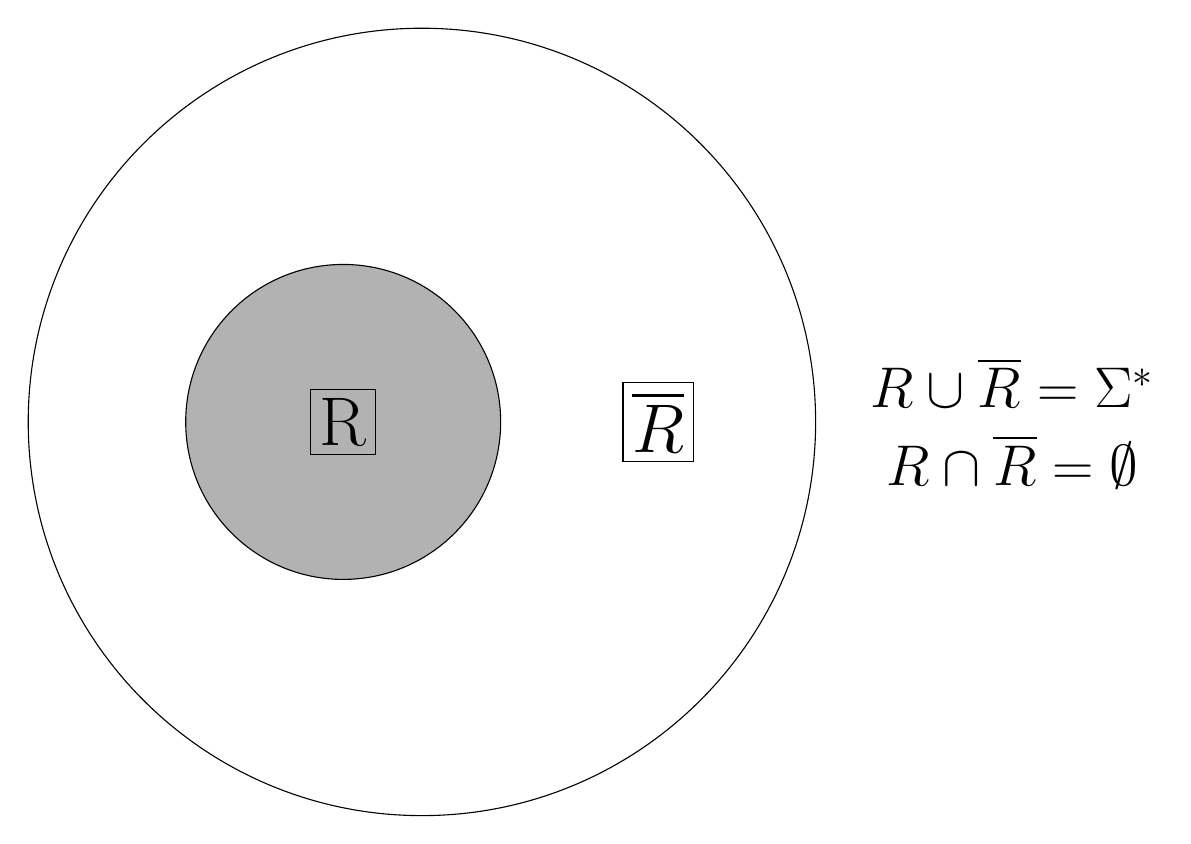
\begin{tikzpicture}
    \filldraw[fill=white, draw=black] (2,2) circle (5cm);
    \node [draw] at (5,2) {\Huge$\overline{R}$};
    \filldraw[fill=gray!60, draw=black] (1,2) circle (2cm);
    \node [draw] at (1,2) {\Huge R};
    \node at (9.5, 2.5) {\huge $R \cup \overline{R} = \Sigma^*$};
    \node at (9.5, 1.5) {\huge $R \cap \overline{R} = \emptyset$};
\end{tikzpicture}}
    \caption{Regular language partition}
    \label{fig:tikz-reg-partition}
\end{figure}

\begin{figure}[!htb]
    \center
    \resizebox{6.5cm}{!}{
    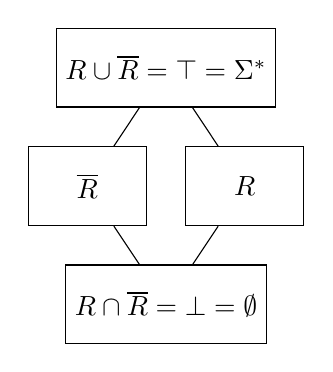
\begin{tikzpicture}
    \usetikzlibrary{calc}
    \node (a) [state] {$R \cup \overline{R} = \top = \Sigma^*$};
    \node (b1) [state, shift={($(a.south)+(1cm, -1cm)$)}] { $R$};
    \node (b2) [state, shift={($(a.south)+(-1cm, -1cm)$)}]{ $\overline{R}$};
    \node (c) [state, shift= {($(a.south) + (0cm, -2.5cm)$)}] { $R \cap \overline{R} = \bot = \emptyset$};
    \draw (a) to (b1);
    \draw (a) to (b2);
    \draw (b1) to (c);
    \draw (b2) to (c);
\end{tikzpicture}}
    \caption{Regular language partition as a lattice}
    \label{fig:tikz-reg-partition-lattice}
\end{figure}

\subsubsection{Abstract tuples}

We define abstract tuples as the product lattice of $\regexs$ and $\uints$ intertwined depending on the schema of the table.
And we define the concretisation function as follows:
\begin{align}
    \concrete_5 &: \bigtimes_{i = 1}^{n}(S_i) \rightarrow \mathcal{P}\left(\bigtimes_{i = 1}^n Z_i \right) \\
    \concrete_5(\ab{e_1}, \ab{e_2}, \dots, \ab{e_n}) &= \concrete_6(\ab{e_1}) \times \concrete_6(\ab{e_2}) \times \dots \times \concrete_6(\ab{e_n})
\end{align}
Where $S_i$ either is $\regexs$ or $\uints$ and $Z_i$ is correspondingly $\strs$ or $\mathbf{NUM}$.

\subsubsection{Single and List values}
When we consider the abstract domain of strings and numbers, we need to consider both single values and lists of values.
We would like to distinguish between single values and lists of values, thus for some set $S$ we define the set $\mathsf{Val} \; S$ inductively as:
\begin{align}
    \inference{}{\bot \in \mathsf{Val} \; S} \quad
    \inference{s \in S}{\mathsf{Single} \; s \in \mathsf{Val} \; S} \quad
    \inference{S' \subseteq S}{\mathsf{List} \; S' \in \mathsf{Val} \; S} \quad
\end{align}
We can define the lattice, $(\mathsf{Val} \; A, \subseteq, \cup, \cap)$, we first define the relation of the lattice:
\begin{align}
    \mathsf{Single} \; s &\sqsubseteq \mathsf{List} \; S \quad
    \text{iff} \; s \in S \\
    \mathsf{Single} \; s_1 &\sqsubseteq \mathsf{Single} \; s_2 \quad
    \text{iff} \; s_1 \sqsubseteq s_2 \\
    \mathsf{List} \; S &\not\sqsubseteq \mathsf{Single} \; s\\
    \mathsf{List} \; S_1 &\sqsubseteq \mathsf{List} \; S_2 \quad
    \text{iff} \; \forall s_1 \in S_1, \; \exists s_2 \in S_2: \; s_1 \sqsubseteq s_2\\
\end{align}

    We define $\cdot \into C_X(S): \ \mathsf{Val} \ S \rightarrow \mathsf{Val} \ C_X(S)$ to be the function that takes some value and inserts it into its cover lattice. \\
    For single elements we use $(\mathsf{Single} \ h) \into C_X(S) = \mathsf{Single}(h\into C_X(S)) \\$
    we say $x \in (\mathsf{Single} \ x') \ \text{iff} \ x = x'.$ \\
    And for a list of elements, we use $(\mathsf{List} \ H) \into C_X(S)=\mathsf{List}(H\into C_X(S))\\$
    we say $x \in (\mathsf{List} \ X) \ \text{iff} \ x \in X.$

We can define the joins and meets of the lattice as follows:
\begin{align}
    \mathsf{Single} \; s \sqcup \mathsf{List} \; S &= \mathsf{List} \; (S\sqcup\left\{ s \right\})\\
    \mathsf{Single} \; s_1 \sqcup \mathsf{Single} \; s_2 &= \mathsf{Single} \; (s \sqcup s )\\
    \mathsf{List} \; S_1 \sqcup \mathsf{List} \; S_2 &= \mathsf{List} \; (S_1 \sqcup S_2)\\
    \mathsf{Single} \; s \sqcap \mathsf{List} \; S &= \mathsf{Single} \; s\\
    \mathsf{List} \; S_1 \sqcap \mathsf{List} \; S_2 &= \mathsf{List} \; (S_1 \sqcap S_2)\\
    \mathsf{Single} \; s_1 \sqcap \mathsf{Single} \; s_2 &= \mathsf{Single} \; (s_1 \sqcap s_2)\\
    \mathsf{List} \ \emptyset \sqcap \mathsf{Single} \ s &= \ \perp
\end{align}
We see that if a list is empty and we look for the meet with a single value, it is equivalent to $\perp$.
As the lattice $(\mathsf{Val} \; A, \subseteq, \cup, \cap)$ is finite, we can use the Kleene fixed-point theorem (see \autoref{thm:kleene_finite}) to prove the termination of our analysis.

We define the concretisation of a variable value as:
\begin{align}
    \concrete_{4a} &: \mathsf{Val} \; \left(C_{X}(S)\right) \rightarrow \mathcal{P}(Z \cup Z^\star) \\
    \concrete_{4a}(\mathsf{Single} \; \ab{s}) &= \concrete_6(\ab{s}) \\
    \concrete_{4a}(\mathsf{List} \; \ab{S'}) &= \bigcup_{n \in \mathbb{N}}\left\{s_1, s_2, \dots, s_n \in Z^n \middle| \forall i \in \{1, 2, \dots, n\} : \exists \ab{s} \in \ab{S'} : s_i \in \concrete_6(\ab{s}) \right\}
\end{align}


\subsubsection{Abstract domain of tables}\label{subsubsec:abstract_domain_of_tables}

We consider a table $t$ as function from the domain of possible tuples in the table $\mathbb{T}$ to the codomain of natural numbers including $0$, $\mathbb{N}$:
\begin{equation}
    t : \mathbb{T} \rightarrow \mathbb{N}.
\end{equation}
The function $t$ describes the number of a given tuple in a table.
We can then consider abstraction over the table $t$ by abstracting either the domain or codomain.
This gives rise to a taxonomy of abstract domains of tables shown in \autoref{tab:taxonomy_of_abstract_domain_of_tables}.
In \autoref{tab:taxonomy_of_abstract_domain_of_tables}, $\mathbb{T}^\#$ denotes an abstract domain of the set of possible tuples $\mathbb{T}$, such that it forms a finite lattice $(\mathbb{T}^\#, \sqsubseteq, \sqcap, \sqcup)$ (and analogous for $\mathbb{N}$).


\begin{table}
    \caption{Taxonomy of abstract domains of tables}
    \centering
    \begin{tabular}{c|l|c}
    Name & Function & Supported \\
    \hline
    \hline
        Bag of tuples & $\mathbb{T} \rightarrow \mathbb{N}$ & \\
        Abstract bag of tuples & $\mathbb{T} \rightarrow \mathbb{N}^\#$ & \\
        Set of tuples & $\mathbb{T} \rightarrow 2$ & \\
        Bag of abstract tuples & $\mathbb{T}^\# \rightarrow \mathbb{N}$ & \\
        Abstract bag of abstract tuples & $\mathbb{T}^\# \rightarrow \mathbb{N}^\#$ & \checkmark \\
        Set of abstract tuples & $\mathbb{T}^\# \rightarrow \{0, some\}$ & \checkmark \\
        Abstract tuple & $\{\cdot\} \rightarrow \mathbb{T}^\#$ & \checkmark \\
    \end{tabular}
    \label{tab:taxonomy_of_abstract_domain_of_tables}
\end{table}

We will only consider abstract bags of abstract tuples, sets of abstract tuples and abstract tuples because of their finite nature.
It should be clear that sets of abstract tuples are just a special case of abstract bags of abstract tuples.
Naturally, these maps all form map lattices.

We define the concretisation of a table as:
\begin{align}
    \concrete_{4d} &: \mathcal{P}\left(\bigtimes_{i = 1}^{n}S_i\right) \rightarrow \mathcal{M}\left(\bigtimes_{i = 1}^n Z_i\right) \\
    \concrete_{4d}(\ab{t}) &= \left\{ t \in \mathcal{M}\left(\bigtimes_{i = 1}^n Z_i\right) \middle|\forall e \in t : \exists \ab{e} \in \ab{t} : e \in \concrete_5(\ab{e}) \right\}
\end{align}

\subsubsection{Abstract environments}

We define an abstract environment $\rho_{\ab{a}} \in \ab{\mathfrak{E}_a}$ mapping application variable names $v_a \in \mathbb{V}_a$ to abstract values, and $\rho_{\ab{d}} \in \ab{\mathfrak{E}_d}$ mapping table names $v_d \in \mathbb{V}_d$ to abstract tables, in symbols:
\begin{align}
    \ab{\mathfrak{E}_a} &= \mathbb{V}_a \rightarrow \mathsf{Val} \; (\regexs) \cup \mathsf{Val} \; (\uints) \\
    \ab{\mathfrak{E}_d} &= \mathbb{V}_d \rightarrow \regexs \cup \uints \cup \regexs \times \regexs \cup \regexs \times \uints \dots \\
    \ab{\mathfrak{E}} &= \ab{\mathfrak{E}_a} \times \ab{\mathfrak{E}_d}
\end{align}

Naturally we define the concretisation functions for environments as:
\begin{align}
    \concrete_2 &: \ab{\mathfrak{E}} \rightarrow \mathcal{P}(\mathfrak{E}) \\
    \concrete_2(\rho_{\ab{d}}, \rho_{\ab{a}}) &= \concrete_{3d}(\rho_{\ab{d}}) \times \concrete_{3a}(\rho_{\ab{a}})
\end{align}
\begin{align}
    \concrete_{3d} &: \ab{\mathfrak{E}_d} \rightarrow \mathcal{P}(\mathfrak{E}_d) \\
    \concrete_{3d}(\rho_{\ab{d}}) &= \left\{ \rho_{a} \in \mathfrak{E}_d \middle| \forall v_d \in \mathbb{V}_d : \rho_d(v_d) \in \concrete_{4d}(\rho_{\ab{d}}(v_d)) \right\}
\end{align}
\begin{align}
    \concrete_{3a} &: \ab{\mathfrak{E}_a} \rightarrow \mathcal{P}(\mathfrak{E}_a) \\
    \concrete_{3a}(\rho_{\ab{a}}) &= \left\{ \rho_{a} \in \mathfrak{E}_a \middle| \forall v_a \in \mathbb{V}_a : \rho_a(v_a) \in \concrete_{4a}(\rho_{\ab{a}}(v_a)) \right\}
\end{align}
And in the same vain we define a concretisation function for sets of environments as:
\begin{align}
    \concrete_1 &: \mathcal{P}(\ab{\mathfrak{E}}) \rightarrow \mathcal{P}(\mathfrak{E}) \\
    \concrete_1(\ab{P}) &= \left\{ (\rho_{d}, \rho_{a}) \in \mathfrak{E} \middle| \exists (\rho_{\ab{d}}, \rho_{\ab{a}}) \in \ab{P} : (\rho_{d}, \rho_{a}) \in \concrete_2(\rho_{\ab{d}}, \rho_{\ab{a}})\right\}
\end{align}


\subsection{Abstract Semantics}

We extend the semantics described in \cite{halder_abstract_2012}, to encompass our taxonomy of abstract tables.

\begin{align*}
    S^\# \llbracket C_{insert}^\# \rrbracket (t) &= S^\# \llbracket insert(\mathbf{v}_d, e^\#) \rrbracket (t) \\
    &= t \sqcup t' \\
    \text{where } E^\# \llbracket e^\# \rrbracket &= t',
\end{align*}

\begin{lemma}
    $S^\# \llbracket C_{insert}^\# \rrbracket$ is monotone.
    %todo
    \todo{Casper says: needs a proving.}
\end{lemma}

\begin{align*}
    E^\# \llbracket R_1 C_{concatenate}^\# R_2 \rrbracket \\
    = E^\# \llbracket R_1 \rrbracket \oplus  E^\# \llbracket R_2 \rrbracket \\
    \text{where } E^\# \llbracket R \rrbracket \text{ is a regular language and }\\
     \oplus \text{ is the concatenation operator.}
\end{align*}
\todo[inline]{Casper says:
    Why $C_{concatenate}^\#$ and not just $\texttt{||}$?
}

\begin{align*}
    E^\# \llbracket C_{bitLength}^\# (R) \rrbracket \\
    = E^\# \llbracket Count(B(R)) \rrbracket \\
    \text{where } B(R) \text{ is the binary representation of }R, \\ \text{ and Count determines the length.}
\end{align*}
\todo[inline]{Casper says:
    Why not just write $\texttt{bit\_length(} R \texttt{)}$, instead of $C_{bitLength}^\#$?
    How would you derive the binary representation of $R$? What is it? How is it computed?
    I think the way I would do this is by finding the shortest $s$ possible string, and the longest possible string $S$ in $R$ and then produce a range $[l(B(s)), l(B(S))]$ where $l$ is the length of a string and $B$ is the binary representation.

}

\begin{align*}
    E^\# \llbracket C_{charLength}^\# (S) \rrbracket \\
    = E^\# \llbracket Count(S) \rrbracket \\
    \text{where } S \text{ is a string and Count determines the length.}
\end{align*}
\todo[inline]{Casper says:
    Same as above? how do you count the lenght of a regular expression?
}

\begin{align*}
    E^\# \llbracket C_{lower}^\# (S) \rrbracket \\
    = E^\# \llbracket MapToLower (S) \rrbracket \\
    \text{where S is a string and } MapToLower \\
    \text{ converts all characters to lowercase.}
\end{align*}
\todo[inline]{Casper says:
    How does $MapToLower$ work, I would suggest a recursive definition.
}

\begin{align*}
    E^\# \llbracket C_{lower}^\# (S) \rrbracket \\
    = E^\# \llbracket MapToUpper (S) \rrbracket \\
    \text{where S is a string and } MapToUpper \\
    \text{ converts all characters to uppercase.}
\end{align*}
\todo[inline]{Casper says:
    Same as above.
}

\begin{align*}
    E^\# \llbracket C_{position}^\# (S_1, in, S_2) \\
    = E^\# \llbracket Position(S_1, in, S_2) \rrbracket \\
    \text{where S is a string and } Position \\
    \text{ returns the position of the first occurrence of } \\
    S_2 \text{ in } S_1.
\end{align*}

\begin{align*}
    E^\# \llbracket C_{subString}^\# (S, I_1, I_2) \rrbracket \\
    = E^\# \llbracket SubString(S, I_1, I_2) \rrbracket \\
    \text{where } S \text{ is a string, } I \text{ are integers, and } \\
    SubString \text{ returns the substring of } S \text{ from } I_1 \text{ to } I_2.
\end{align*}

\begin{align*}
    E^\# \llbracket C_{trim}^\# (S_1 from S_2) \rrbracket \\
    = E^\# \llbracket Trim(S_1, S_2) \rrbracket \\
    \text{where } S_1 \text{ and } S_2 \text{ are strings, and }\\
    Trim \text{ removes all occurrences of } S_2 \text{ from } S_1.
\end{align*}

\todo[inline]{Casper says:
    For the tree definitions above a definition should be give for position, substring and trim.
    We should be able to implement the abstract semantics by following the semantics above.
}



\subsection{Abstract Interpretation of belongs}
To provide a precise definition of the belongs function, envision a lattice composed of partitions of a language. We aim to identify the most precise partition that encompasses a given expression. In essence, we seek to pinpoint which element in the lattice accurately describes the expression's location. Simply stating that it resides somewhere within the entire set would lack practicality.

Partitions within this lattice may overlap, symbolizing intersections of languages. The lattice itself is complete, with the top element representing the entire set of languages, and the bottom element indicating the empty set.

Navigating this lattice involves starting from the top and descending until we reach a point where no partitions cover the expression. At this juncture, we have identified the most precise set of partitions that encompass the expression.

$ belongs(x)=\bigsqcap\{x' \mid x \sqsubseteq x', x' \in X\} $
Taking an expression $x$, we seek to identify the most precise partition that encompasses it. We do this by finding the greatest lowerbound of all partitions that contain $x$.




    \printglossary[type=\acronymtype]

    \printbibliography

    \appendices % You can use \appendix if you only have a single appendix
    %! Author = Runge
%! Date = 29-12-2023

\section{Proof of theorem \ref{thm:partition}}

\begin{lemma}\label{lem:finite-partition}
    For a non-complete lattice $(S, \sqsubseteq, \sqcup, \sqcap)$ and a finite non-empty subset $X \subseteq S$ where $\bigsqcup X = \top$, $p_X(S)$ is finite.
\end{lemma}

\begin{proof}
    \pf\
    \step{base-case}{\case{$X = \{x\}$}}
    \begin{proof}
        \step{}{$x = \top$}
        \begin{proof}
            \pf\ By the assumption $\bigsqcup \{x\} = \top$.
        \end{proof}
        \step{}{$p_X(S) = \{\top\}$}
        \begin{proof}
            \pf\ By the definition of $p$: $\top \in p_X(S)$, $\top \sqcup \top = \top \in p_X(S)$ and $\top \sqcap \top = \top \in p_X(S)$.
        \end{proof}
    \end{proof}
    \step{inductive-case}{\case{$|X| > 1$}}
    \begin{proof}
        \assume{$p_X(S)$ is finite.}
        \prove{$p_{(X \cup \{y\})}(S)$ is finite, when $y \in S \setminus X$.}
        \pf\ It should be obvious that $\forall x \in p_X(S) : x \in p_{(X \cup \{y\})}(S)$.
        By the definition of $p$ $\forall x \in p_X(S) : x \sqcup y \in p_{(X \cup \{y\})}(S)$ (analogous for $\sqcap$).
        Further $(x \sqcup y) \sqcup y = x \sqcup y$ (analogous for $\sqcap$), and $(x \sqcup y) \sqcap y = y$, and $(x \sqcap y) \sqcup y = y$.
        This means that $\forall x \in p_X(S) : x \in p_{(X \cup \{y\})}(S) \land (x \sqcup y) \in p_{(X \cup \{y\})}(S)$ and no more elements are in $p_{(X \cup \{y\})}(S)$, thus $p_{(X \cup \{y\})}(S)$ is finite.
    \end{proof}
    \qedstep
    \begin{proof}
        \pf\ By induction, \stepref{base-case} and \stepref{inductive-case}.
    \end{proof}
\end{proof}

\partition*

\begin{proof}
    \pf\
    \assume{
        $(S, \sqsubseteq, \sqcup, \sqcap)$ is a non-complete lattice and $X \subset S$ and $\bigsqcup X = \top$.
    }
    \prove{
        $(p_X(S), \sqsubseteq, \sqcup, \sqcap) \text{ is a finite and complete lattice}$.
    }
    \step{complete}{A nonempty finite lattice is a complete lattice.}
    \begin{proof}
        \pf\ Know property \cite{moller_statitc_nodate}.
    \end{proof}
    \step{lattice}{$(p_X(S), \sqsubseteq, \sqcup, \sqcap)$ is a lattice.}
    \begin{proof}
        \step{poset}{$p_X(S)$ is a poset}
        \begin{proof}
            \step{poset-subset}{The subset of a poset is a poset under the same ordering relation.}
            \begin{proof}
                \pf\ Know property.\todo{source missing}
            \end{proof}
            \step{partition-subset}{$p_X(S) \subset S$}
            \begin{proof}
                \pf\ By the definition of a partition and lattices.
            \end{proof}
            \qedstep
            \begin{proof}
                \pf\ By \stepref{poset-subset} and \stepref{partition-subset}.
            \end{proof}
        \end{proof}
        \step{capcup}{$\forall x, y \in p_X(S) : x \sqcup y \in p_X(S) \land x \sqcap y \in p_X(S)$}
        \begin{proof}
            \pf\ By the definition of $p_X(S)$.
        \end{proof}
        \qedstep
        \begin{proof}
            \pf\ By \stepref{poset} and \stepref{capcup}.
        \end{proof}
    \end{proof}
    \step{finite}{$p_X(S)$ is finite.}
    \begin{proof}
        \pf\ By \autoref{lem:finite-partition}.
    \end{proof}
    \qedstep
    \begin{proof}
        \pf\ By \stepref{complete}, \stepref{lattice} and \stepref{finite}.
    \end{proof}
\end{proof}

\section{Proof of theorem \ref{thm:csql}}

\csql*

\begin{proof}
    \pf\
    \suffices{To show that any function of the form $F(X)=\{f(x)|x\in X\}$ is monotone,
        as $S\llbracket C_{sql}\rrbracket(\widehat{P})$ is a special case of this type of function in which $X\in \widehat{P}(A)$ where $(\widehat{P}(A),\subseteq)$.}
    \step{monotone}{$F(X)=\{f(x)|x\in X\}$ is monotone}
    \begin{proof}
        \pf\ Assume $X\subseteq X'$. If $x\in X$ then $x \in X'$. This means that for $f(x)\in F(X)$, $f(x)\in F(X')$ because $x\in X'$
    \end{proof}
    \qedstep
    \begin{proof}
        \pf\ By \stepref{monotone}
    \end{proof}
\end{proof}

\section{Proof of \autoref{thm:galios}}\label{sec:galois}

% \galois

\begin{proof}
    \pf\
    \step{meet-morphism-1}{$\concrete_1$ is a meet morphism.}
    \begin{proof}
        \pf\
        \begin{align}
            \concrete_1 \left( \bigcap \mathcal{R} \right)
            &=  \mathcal{L} \left( \bigcap \mathcal{R} \right)\\
            &=  \bigcap_{R \in \mathcal{R}} \mathcal{L} \left( R \right)\\
            &=  \bigcap_{R \in \mathcal{R}} \concrete_1 \left( R \right)
        \end{align}
    \end{proof}
    \step{meet-morphism-2}{$\concrete_2$ is a meet morphism.}
    \begin{proof}
        \pf\
        \begin{align}
            \concrete_2 \left( \bigsqcap_{i = 1}^m (e_{i1}^\#, e_{i2}^\#, \dots, e_{in}^\#) \right)
            &= \concrete_2 \left( \bigsqcap_{i = 1}^m e_{i1}^\#, \bigsqcap_{i = 1}^m e_{i2}^\#, \dots, \bigsqcap_{i = 1}^m e_{in}^\# \right) \\
            &= \bigtimes_{j = 1}^n \concrete_1 \left( \bigsqcap_{i = 1}^m e_{ij}^\# \right) \\
            &= \bigtimes_{j = 1}^n \bigcap_{i = 1}^m \concrete_1 (e_{ij}^\#) \text{ as $\concrete_1$ is a meet morphism by \stepref{meet-morphism-1}} \\
            &= \bigcap_{i = 1}^m \bigtimes_{j = 1}^n \concrete_1 (e_{ij}^\#) \\
            &= \bigcap_{i = 1}^m \concrete_2 (e_{i1}^\#, e_{i2}^\#, \dots, e_{in}^\#) \\
        \end{align}
    \end{proof}
    \step{meet-morphism-3}{$\concrete_3$ is a meet morphism.}
    \begin{proof}
        \pf\
        \pflet{$T^\# = \left\{ t^\#_1, t^\#_2, \dots, t^\#_n \right\}$}
        \begin{align}
            t \in \concrete_3\left(\bigsqcap T^\#\right)
            &\iff \\
            \forall e^\# \in \mathbb{T}^\# : \left( \sum_{e \in \concrete_2\left(e^\#\right)} t\left(e\right) \right) \in \concrete_2\left(\left(\bigsqcap T^\#\right)\left(e^\#\right)\right)
            &\equiv
            \forall e^\# \in \mathbb{T}^\# : \left( \sum_{e \in \concrete_2\left(e^\#\right)} t\left(e\right) \right) \in \concrete_2\left(\bigsqcap_{t^\# \in T^\#} t^\#\left(e^\#\right)\right) \\
            &\equiv
            \forall e^\# \in \mathbb{T}^\# : \left( \sum_{e \in \concrete_2\left(e^\#\right)} t\left(e\right) \right) \in \bigcap_{t^\# \in T^\#} \concrete_2\left(t^\#\left(e^\#\right)\right) \\
            &\equiv
            \forall e^\# \in \mathbb{T}^\# : \forall t^\# \in T^\# : \left( \sum_{e \in \concrete_2\left(e^\#\right)} t\left(e\right) \right) \in \concrete_2\left(t^\#\left(e^\#\right)\right) \\
            &\equiv
            \forall t^\# \in T^\# : \forall e^\# \in \mathbb{T}^\# : \left( \sum_{e \in \concrete_2\left(e^\#\right)} t\left(e\right) \right) \in \concrete_2\left(t^\#\left(e^\#\right)\right) \\
            &\iff
            t \in \bigcap_{t^\# \in T^\#} \concrete_3\left(t^\#\right)
        \end{align}
    \end{proof}
    \step{meet-morphism-4}{$\concrete_4$ is a meet morphism.}
    \begin{proof}
        \pf\ Analogous to \stepref{meet-morphism-2}.
    \end{proof}
    \step{meet-morphism-5}{$\concrete_5$ is a meet morphism.}
    \begin{proof}
        \pf\ The proof of $\concrete_5(\bigsqcap D^\#) = \bigsqcap_{\rho_{d^\#} \in D^\#} \concrete_5(\rho_{d^\#})$ is analogous to the one below.
        \pflet{
            $P^\# = \{ \rho_{t_1^\#}, \rho_{t_2^\#}, \dots, \rho_{t_n^\#} \}$ \\
            $T^\# = \{ t_1^\#, t_2^\#, \dots, t_n^\# \}$
        }
        \begin{align}
            \concrete_5 \left( \bigsqcap P^\# \right) &=  \concrete_5 \left( \rho_{\bigsqcap T^\#} \right) \\
            &= \left\{ \left. \env{t} \ \middle| \ t \in \concrete_3 \left( \bigsqcap T^\# \right) \right. \right\}
        \end{align}
        \begin{align}
            \bigcap_{\rho_{t^\#} \in P^\#} \concrete_5 \left( \rho_{t^\#} \right) &= \bigcap_{t^\# \in T^\#} \concrete_5 \left( \rho_{t^\#} \right) \\
            &= \bigcap_{t^\# \in T^\#} \left\{ \left. \env{t} \ \middle| \ t \in \concrete_3 \left( t^\# \right) \right. \right\}
        \end{align}
        \begin{align}
            \rho_t \in \concrete_5 \left( \bigsqcap P^\# \right)
            &\iff \\
            t \in \concrete_3 \left( \bigsqcap T^\# \right)
            &\equiv
            t \in \bigcap_{t^\# \in T^\#} \concrete_3 \left(t^\# \right) \\
            &\equiv
            \forall t^\# \in T^\# : t \in \concrete_3 \left(t^\# \right) \\
            &\iff \bigsqcap_{\rho_{t^\#} \in P^\#} \concrete_5 \left( \rho_{t^\#} \right)
        \end{align}
    \end{proof}
    \qedstep
    \begin{proof}
        \pf\ By \autoref{thm:galoispre} and \stepref{meet-morphism-5}.
    \end{proof}
\end{proof}







\end{document}
